\documentclass{article}

\usepackage[%
  papersize={18cm,16cm},
  hmargin=0cm,%
  vmargin=0cm,%
  head=0cm,%
  headsep=0pt,%
  foot=0cm%
  ]{geometry}

\usepackage{etex}       % changes how LaTex allocates registers (needed for pgfplots)
\usepackage{pgfplots}   % for drawing plots
\usepackage{charter}    % sets font as bitstream charter
\usepackage{filecontents}
\usetikzlibrary{patterns,external}
\usepgfplotslibrary{colormaps}

\pgfplotsset{
  compat=1.9,
  colormap={heatto}{[1pt]
    rgb255(0pt)=(255, 255, 240);
    rgb255(5pt)=(255, 255, 0);
    rgb255(600pt)=(255, 180, 0);
    rgb255(1200pt)=(255, 80, 0);
    rgb255(1799pt)=(255, 0, 0);
    rgb255(1800pt)=(0, 0, 0);
  },
  heat/.style={
    view={0}{90},
    font=\scriptsize,
    colormap name=heatto,
    point meta min=0,
    point meta max=1800000,
    xtick={0.5,1.5,2.5,3.5,4.5,5.5,6.5},
    ytick={0.5,1.5,2.5,3.5,4.5,5.5,6.5},
    xticklabels={},
    yticklabels={},
    ylabel style={rotate=-90,text width=20pt},
    xtick style={draw=none},
    ytick style={draw=none},
    title style={font=\normalsize},
    width=3.5995cm,
    height=3.5995cm},
  mat/.style={
    surf,
    shader=flat corner,
    draw=black,
    line width=0.01pt,
  },
}

\newcommand{\MTSA}{{\scshape mtsa}}
\newcommand{\SUP}{{\scshape supremica}}
\newcommand{\MBP}{{\scshape mbp}}
\newcommand{\MYND}{{\scshape mynd}}
\newcommand{\RA}{{\scshape dcs-ra}}
\newcommand{\RAnew}{{\scshape dcs2-ra}}

\pagestyle{empty}
  
\begin{document}
\begin{figure}
\centering
\begin{tikzpicture}
\matrix {
% TL %
\begin{axis}[heat,yticklabels={0,1,2,3,4,5,6},title=\MTSA]
  \addplot3[mat] table[z index=2] {data/TL.dat}; \end{axis} &  % MTSA (2)
\begin{axis}[heat,title=\SUP] 
  \addplot3[mat] table[z index=3] {data/TL.dat}; \end{axis} &  % SUPREMICA (3)
\begin{axis}[heat,title=\MBP] 
  \addplot3[mat] table[z index=4] {data/TL.dat}; \end{axis} &  % MBP (4)
\begin{axis}[heat,title=\MYND] 
  \addplot3[mat] table[z index=6] {data/TL.dat}; \end{axis} &  % MYND (6)
\begin{axis}[heat,title=\RA] 
  \addplot3[mat] table[z index=3] {data/TL-dcs.dat}; \end{axis} & % RA (3)
\begin{axis}[heat,title=\RAnew]
  \addplot3[mat] table[z index=3] {data/TL-dcs2.dat}; \end{axis} \\ % RA new
% DP %
\begin{axis}[heat,yticklabels={0,1,2,3,4,5,6}]
  \addplot3[mat] table[z index=2] {data/DP.dat}; \end{axis} &  % MTSA (2)
\begin{axis}[heat]
  \addplot3[mat] table[z index=3] {data/DP.dat}; \end{axis} &  % SUPREMICA (3)
\begin{axis}[heat]
  \addplot3[mat] table[z index=4] {data/DP.dat}; \end{axis} &  % MBP (4)
\begin{axis}[heat]
  \addplot3[mat] table[z index=6] {data/DP.dat}; \end{axis} &  % MYND (6)
\begin{axis}[heat]
  \addplot3[mat] table[z index=3] {data/DP-dcs.dat}; \end{axis} & % RA (3)
\begin{axis}[heat]
  \addplot3[mat] table[z index=3] {data/DP-dcs2.dat}; \end{axis} \\ % RA new
% CM %
\begin{axis}[heat,yticklabels={0,1,2,3,4,5,6}]
  \addplot3[mat] table[z index=2] {data/CM.dat}; \end{axis} &  % MTSA (2)
\begin{axis}[heat]
  \addplot3[mat] table[z index=3] {data/CM.dat}; \end{axis} &  % SUPREMICA (3)
\begin{axis}[heat]
  \addplot3[mat] table[z index=4] {data/CM.dat}; \end{axis} &  % MBP (4)
\begin{axis}[heat]
  \addplot3[mat] table[z index=6] {data/CM.dat}; \end{axis} &  % MYND (6)
\begin{axis}[heat]
  \addplot3[mat] table[z index=3] {data/CM-dcs.dat}; \end{axis} & % RA (3)
\begin{axis}[heat]
  \addplot3[mat] table[z index=3] {data/CM-dcs2.dat}; \end{axis} \\ % RA new
% AT %
\begin{axis}[heat,yticklabels={0,1,2,3,4,5,6}]
  \addplot3[mat] table[z index=2] {data/AT.dat}; \end{axis} &  % MTSA (2)
\begin{axis}[heat]
  \addplot3[mat] table[z index=3] {data/AT.dat}; \end{axis} &  % SUPREMICA (3)
\begin{axis}[heat]
  \addplot3[mat] table[z index=4] {data/AT.dat}; \end{axis} &  % MBP (4)
\begin{axis}[heat]
  \addplot3[mat] table[z index=6] {data/AT.dat}; \end{axis} &  % MYND (6)
\begin{axis}[heat]
  \addplot3[mat] table[z index=3] {data/AT-dcs.dat}; \end{axis} & % RA (3)
\begin{axis}[heat]
  \addplot3[mat] table[z index=3] {data/AT-dcs2.dat}; \end{axis} \\ % RA new
% BW %
\begin{axis}[heat,yticklabels={0,1,2,3,4,5,6}]
  \addplot3[mat] table[z index=2] {data/BW.dat}; \end{axis} &  % MTSA (2)
\begin{axis}[heat]
  \addplot3[mat] table[z index=3] {data/BW.dat}; \end{axis} &  % SUPREMICA (3)
\begin{axis}[heat]
  \addplot3[mat] table[z index=4] {data/BW.dat}; \end{axis} &  % MBP (4)
\begin{axis}[heat]
  \addplot3[mat] table[z index=6] {data/BW.dat}; \end{axis} &  % MYND (6)
\begin{axis}[heat]
  \addplot3[mat] table[z index=3] {data/BW-dcs.dat}; \end{axis} & % RA (3)
\begin{axis}[heat]
  \addplot3[mat] table[z index=3] {data/BW-dcs2.dat}; \end{axis} \\ % RA new
% TA %
\begin{axis}[heat,yticklabels={0,1,2,3,4,5,6},xticklabels={0,1,2,3,4,5,6}]
  \addplot3[mat] table[z index=2] {data/TA.dat}; \end{axis} &  % MTSA (2)
\begin{axis}[heat,xticklabels={0,1,2,3,4,5,6}]
  \addplot3[mat] table[z index=3] {data/TA.dat}; \end{axis} &  % SUPREMICA (3)
\begin{axis}[heat,xticklabels={0,1,2,3,4,5,6}]
  \addplot3[mat] table[z index=4] {data/TA.dat}; \end{axis} &  % MBP (4)
\begin{axis}[heat,xticklabels={0,1,2,3,4,5,6}]
  \addplot3[mat] table[z index=6] {data/TA.dat}; \end{axis} &  % MYND (6)
\begin{axis}[heat,xticklabels={0,1,2,3,4,5,6}]
  \addplot3[mat] table[z index=3] {data/TA-dcs.dat}; \end{axis} & % RA (3)
\begin{axis}[heat,xticklabels={0,1,2,3,4,5,6}]
  \addplot3[mat] table[z index=3] {data/TA-dcs2.dat}; \end{axis} \\ % RA new
};
% LABELS %
\node (n) at (0.15,-7.6) {\footnotesize Value of $n$};
\node[rotate=90] (k) at (-7.3,-0.1) {\footnotesize Value of $k$};
\node (tl) at (7.4,5.7)   {\small TL};
\node (dp) at (7.4,3.35)  {\small DP};
\node (cm) at (7.4,1.05)  {\small CM};
\node (at) at (7.4,-1.25) {\small AT};
\node (bw) at (7.4,-3.6)  {\small BW};
\node (ta) at (7.4,-5.9)  {\small TA};
\end{tikzpicture}
% COLOR BAR %
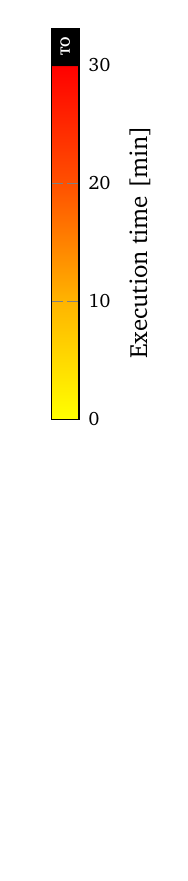
\begin{tikzpicture}
\begin{axis}[
  hide axis,
  height=12.5cm,
  colorbar,
  colorbar style={
    colormap name=heatto,
    height=4.5cm,
    width={10pt},
    font={\small},
    ticklabel style={font=\scriptsize},
    ytick={0,0.333,0.666,1},
    yticklabels={0,10,20,30},
    ylabel={Execution time [min]},
  },
] \end{axis}
\node[text=white,shape=rectangle,fill=black,rotate=90,minimum height=10.4pt,anchor=south east] at (1.7425,11.4) {\tiny \bf TO};
\end{tikzpicture}
\end{figure}

\end{document}
